% Standalone version of Fig. 1 from paper/main.tex, restyled for slides.
% Build: xelatex -output-directory=... pipeline.tex  -> pdftocairo -svg
%
% One loop, run twice. Round 1 is the expert demonstrations, round 2 the
% policy's own rollouts; everything downstream of the data node is shared, which
% is exactly the point — the critic is trained and the frames are labelled the
% same way in both rounds. SnapFlow is deliberately absent: it is a distillation
% step applied to a finished policy, not part of this loop.
\documentclass[tikz,border=4pt]{standalone}
\usepackage{amsmath,amssymb}
\usetikzlibrary{arrows.meta,positioning,calc,fit,backgrounds,shapes.geometric}

\newcommand{\pf}{\ensuremath{f^{+}}}

\begin{document}
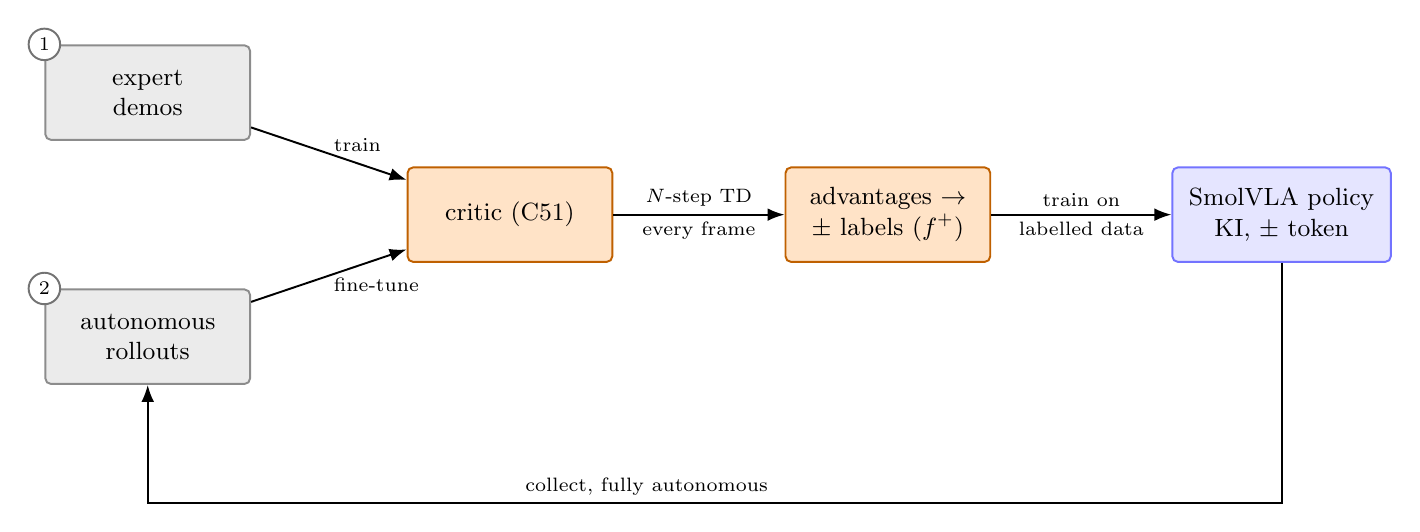
\begin{tikzpicture}[font=\small, >=Latex, line width=0.7pt,
  box/.style={draw, rounded corners=2pt, align=center, inner sep=6pt,
              minimum height=12mm, minimum width=26mm},
  data/.style={box, fill=black!8,   draw=black!45},
  pol/.style={box,  fill=blue!10,   draw=blue!55},
  crit/.style={box, fill=orange!22, draw=orange!75!black},
  rnd/.style={circle, draw=black!55, fill=white, inner sep=0.6pt,
              font=\scriptsize, minimum size=4mm},
  lbl/.style={font=\scriptsize, inner sep=2.5pt}]

\node[data] (demos)  at (0,1.55)    {expert\\demos};
\node[data] (roll)   at (0,-1.55)   {autonomous\\rollouts};
\node[crit] (critic) at (4.6,0)     {critic (C51)};
\node[crit] (labels) at (9.4,0)     {advantages $\to$\\$\pm$ labels (\pf)};
\node[pol]  (policy) at (14.4,0)    {SmolVLA policy\\KI, $\pm$ token};

% Round 1: the critic is trained on the demonstrations, which are then labelled
% and used to pre-train an already advantage-conditioned policy.
\draw[->] (demos) -- node[lbl, above right=-2pt and -1pt]{train} (critic);
% Round 2: the same critic is fine-tuned on the rollouts the policy collected.
\draw[->] (roll)  -- node[lbl, below right=-2pt and -1pt]{fine-tune} (critic);

% Which round each data source belongs to. Everything to the right of the critic
% is shared, so the badges belong on the data and nowhere else.
\node[rnd] at (demos.north west) {1};
\node[rnd] at (roll.north west)  {2};

\draw[->] (critic) -- node[lbl, above]{$N$-step TD}
                      node[lbl, below]{every frame} (labels);
\draw[->] (labels) -- node[lbl, above]{train on}
                      node[lbl, below]{labelled data} (policy);

% The loop that makes round 2 possible at all: no teleoperation, no human in it.
\draw[->] (policy.south) -- ++(0,-3.05) -| node[lbl, above, pos=0.28]{collect,
          fully autonomous} (roll.south);
\end{tikzpicture}
\end{document}
